\documentclass[a4paper,12pt]{article}

\usepackage[utf8]{inputenc}
\usepackage[spanish]{babel}
\usepackage{graphicx}
\usepackage{geometry}
\usepackage{datetime}
\usepackage{titlesec}
\usepackage{fancyhdr}
\usepackage{parskip}

% Márgenes
\geometry{left=3cm, right=2.5cm, top=3cm, bottom=3cm}

\begin{document}

% Incluir carátula
\begin{titlepage}
    \begin{center}
        {\LARGE \textbf{Universidad Nacional de Córdoba}}\\[1.5cm]

        
\includegraphics[scale=0.4]{images/logo2.png}\\[1.5cm]

        {\large Facultad de Ciencias Exactas, Físicas y Naturales}\\
        {\large Escuela de Electrónica y Computacion}\\[1cm]

        \rule{\linewidth}{0.5mm}\\[0.4cm]
        {\Large \textbf{Cátedra de Sistemas de Computacion}}\\[0.3cm]
        {\LARGE \textbf{Trabajo de Laboratorio 3}}\\[0.3cm]

        \rule{\linewidth}{0.5mm}\\[1cm]

        \begin{flushleft}
        {\large 
            \textbf{Profesor Titular:} Ing. Javier Alejandro JORGE\\
            \textbf{Profesor Adjunto:} -\\[0.5cm]
            \textbf{Integrantes:}\\
            Trucchi, Genaro\\
            Trachtta, Agustin\\
            Rodriguez, Mateo\\
        }
        \end{flushleft}

        \vfill

        {\large \today}
    \end{center}
\end{titlepage}


% Comienza el contenido real del informe
\section{Resumen}
Aquí va el resumen del trabajo.

\section{Introducción}
Aquí va la introducción al informe.

\newpage

\section{Resultados}
Aquí se detallan los resultados del laboratorio.

\subsection{Resultados PC Agustin}

\subsubsection*{1. Uso cotidiano de la PC}
Utilizo mi PC principalmente para jugar videojuegos, tanto singleplayer como multiplayer. Me interesa obtener una buena experiencia visual y de fluidez, así como minimizar la latencia. También presto atención al rendimiento térmico y a la estabilidad del sistema durante sesiones largas de juego. El sistema operativo es Windows, y utilizo herramientas como MSI Afterburner y GeForce Experience.

\subsubsection*{2. Tareas y benchmarks representativos}

A continuación se presenta una tabla con distintos aspectos del gaming y los benchmarks o herramientas que mejor los representan.

\begin{center}
\begin{tabular}{|p{7cm}|p{7cm}|}
\hline
\textbf{Tarea / Escenario} & \textbf{Benchmarks} \\
\hline
Jugar videojuegos (rendimiento FPS y calidad gráfica) & Benchmarks sintéticos de GPU como \textbf{3DMark} \\
\hline
Jugar videojuegos (latencia) & Para latencia de entrada: \textbf{NVIDIA Reflex} (si es compatible con el juego) o herramientas como \textbf{CapFrameX} para analizar frame times. Para latencia de red: pruebas de ping y jitter a servidores de juego o valores integrados en juegos online. \\
\hline
\end{tabular}
\end{center}

\subsubsection*{3. Análisis de prueba con 3DMark}

Se realizó una prueba con la herramienta 3DMark para evaluar el rendimiento de la GPU y la CPU durante una carga gráfica sostenida.

\begin{itemize}
  \item \textbf{GPU:} NVIDIA GeForce GTX 1050 Ti
  \item \textbf{CPU:} Intel Core i3-9100F
  \item \textbf{Resolución:} 1920×1080
  \item \textbf{Sistema operativo:} Windows 10
\end{itemize}

Durante la prueba, se observaron los siguientes comportamientos:

\begin{itemize}
  \item La \textbf{GPU se mantuvo al 100\% de carga} durante toda la ejecución del test, lo que indica que es el principal limitante de rendimiento en este sistema.
  \item Se registró una temperatura promedio de \textbf{59.34°C} en la GPU, dentro de valores normales para este tipo de uso.
  \item La \textbf{CPU tuvo una carga media del 65\%}, lo cual indica que no está siendo un cuello de botella en este escenario particular.
  \item El \textbf{framerate promedio fue de 20 FPS}, lo que indica que el sistema puede ejecutar cargas gráficas intensas, pero con una fluidez limitada. Para juegos exigentes, es recomendable usar configuraciones gráficas medias o bajas para mantener los 60 FPS.
\end{itemize}

\hspace*{-1.2cm}
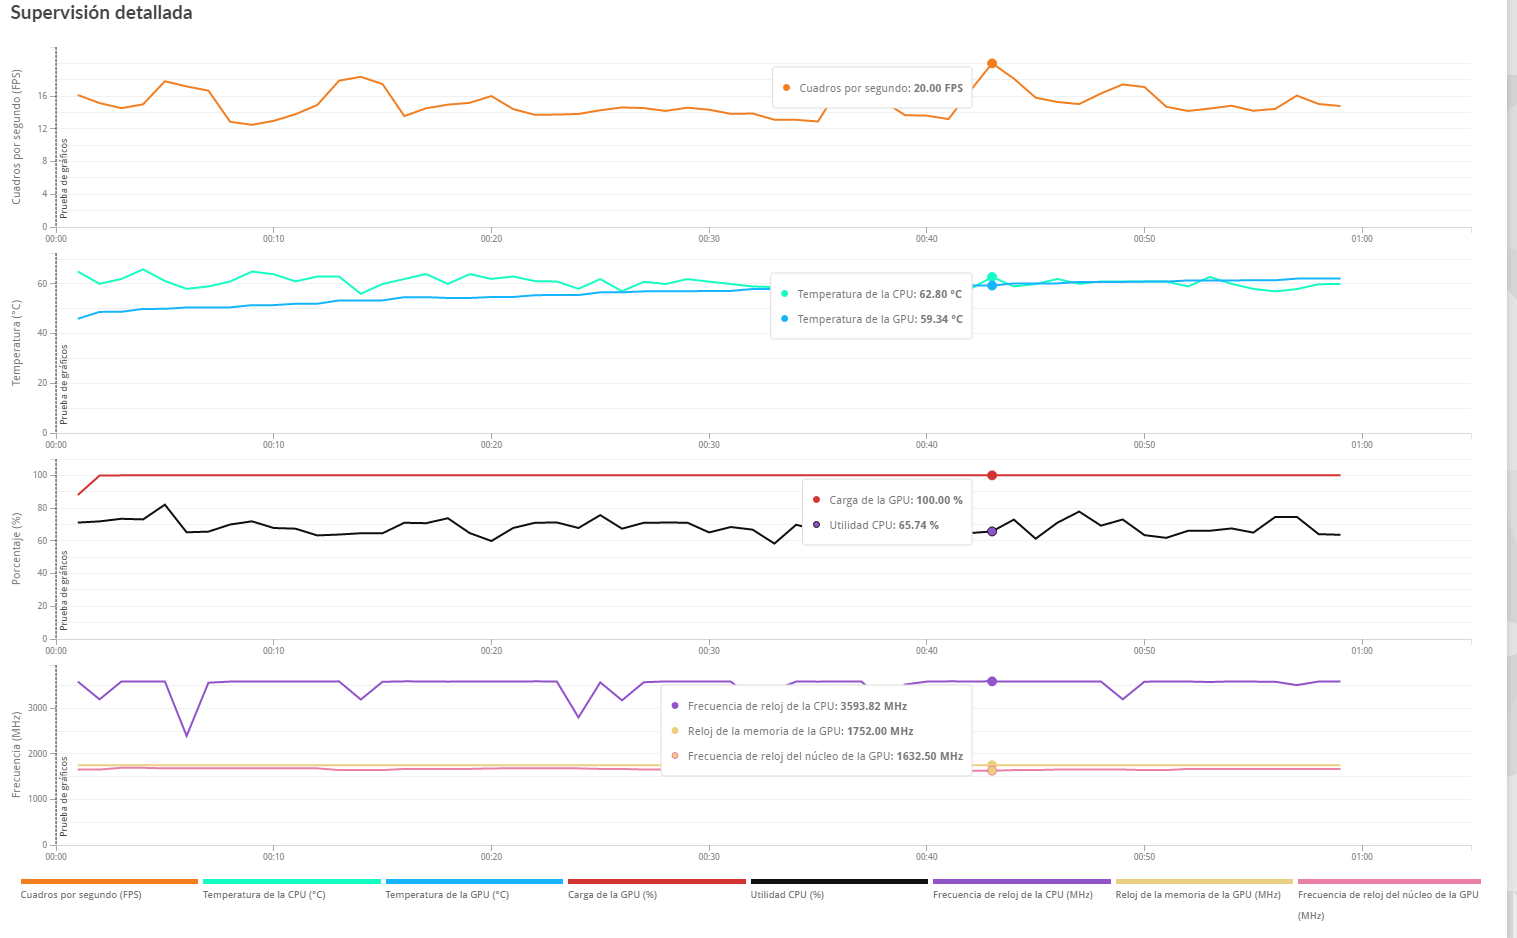
\includegraphics[width=1.2\textwidth]{img/3dmarkagu.png}

\begin{center}
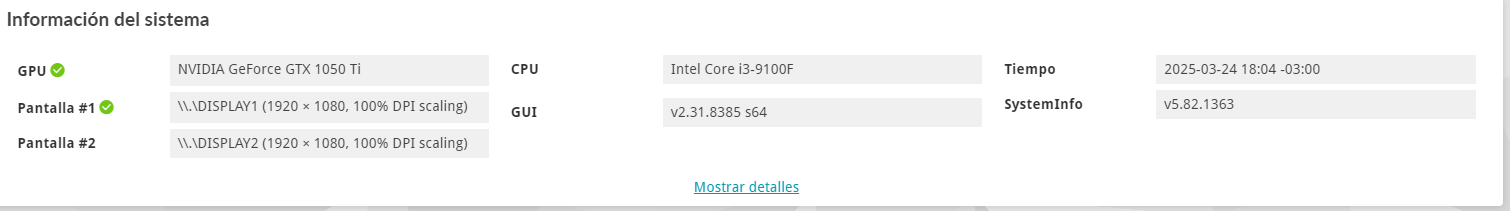
\includegraphics[width=1.1\textwidth]{img/informacionpcagu.png}
\end{center}

Este resultado es útil como línea base para comparar futuros upgrades. Si se busca mejorar el rendimiento en juegos, el cambio más impactante sería actualizar la GPU.

\subsubsection*{5. Medición de latencia de red con PingPlotter}

Para analizar la latencia de red, se utilizó la herramienta \textbf{PingPlotter}, apuntando al servidor de Riot Games (\texttt{riotgames.com}). Esta herramienta permite visualizar el comportamiento de la conexión en cada salto hasta el destino final, incluyendo pérdida de paquetes (packet loss), tiempo de ida y vuelta (ping) y jitter.

\begin{itemize}
  \item \textbf{IP objetivo:} 104.104.37.123
  \item \textbf{Duración de la prueba:} 10 minutos
  \item \textbf{Promedio de latencia:} 20.7 ms
  \item \textbf{Mínimo:} 14.0 ms \hspace{1cm} \textbf{Máximo (Cur):} 16.3 ms
  \item \textbf{Pérdida de paquetes:} Se observa pérdida parcial en los primeros saltos, pero no afecta al destino final.
\end{itemize}

La siguiente imagen muestra los resultados detallados de la prueba:

\begin{center}
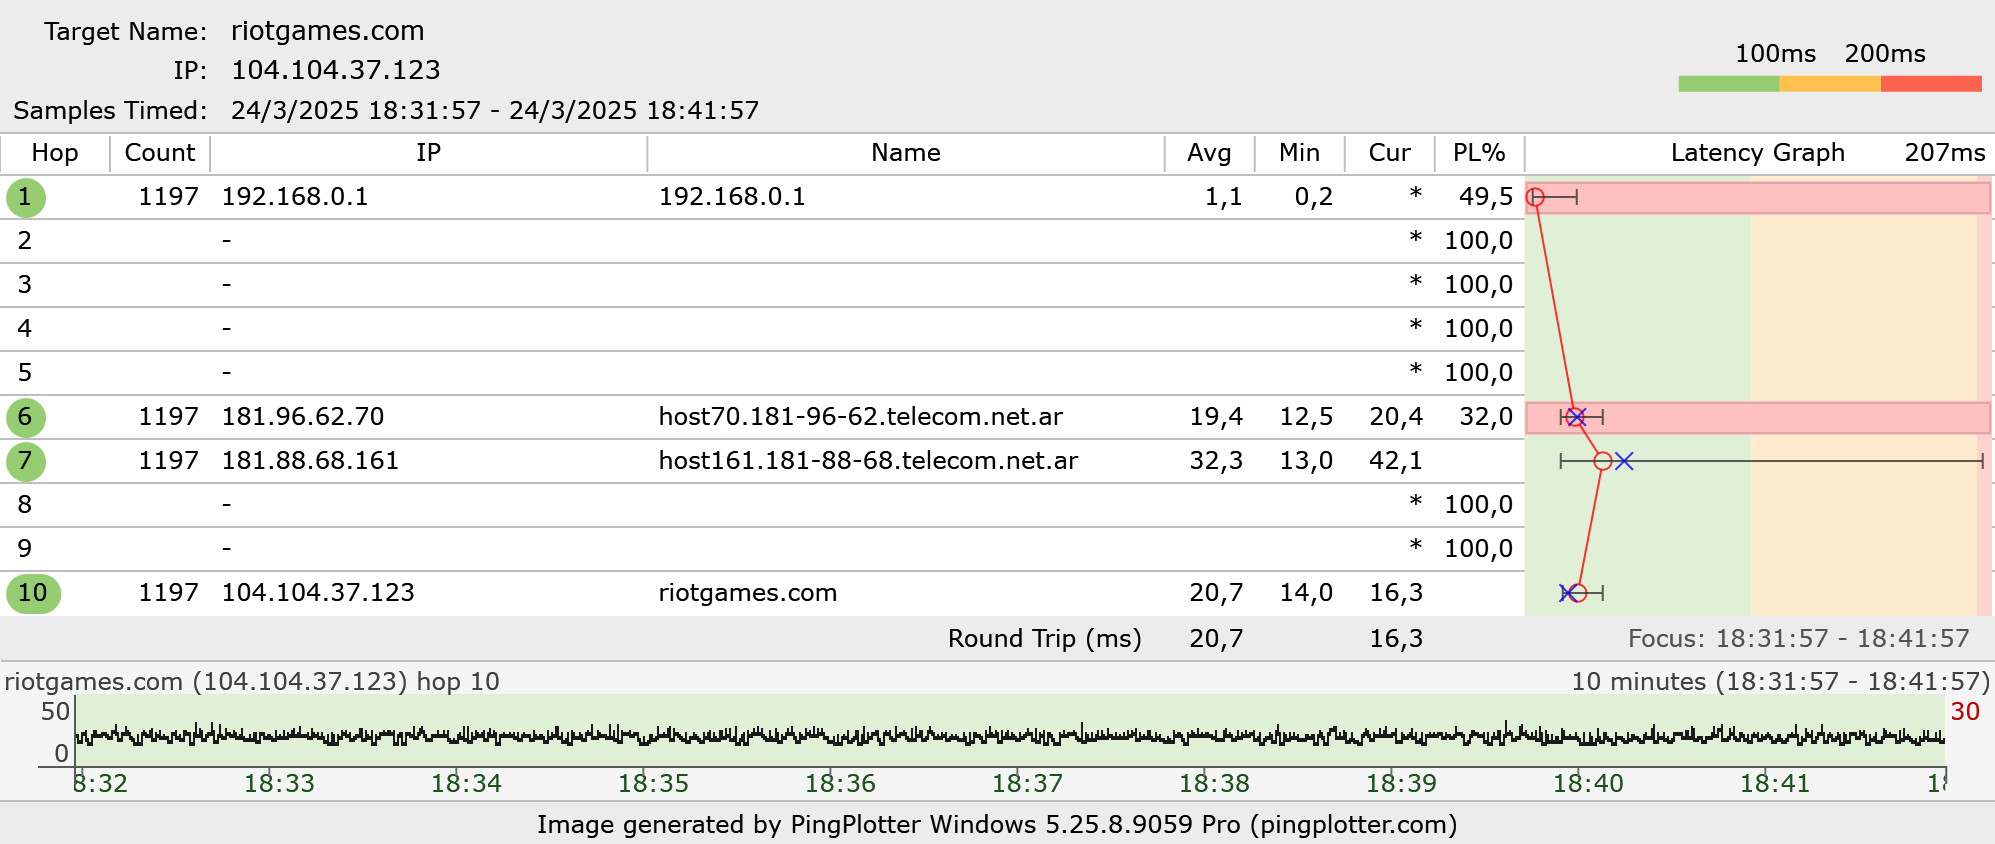
\includegraphics[width=1.05\textwidth]{img/latenciaagu.png}
\end{center}

Se observa que el \textbf{servidor de Riot Games responde con una latencia baja y estable}, lo cual es ideal para juegos en línea. La pérdida de paquetes en los primeros nodos suele deberse a equipos intermedios que priorizan tráfico real y no responden todos los pings; no representa un problema si no llega al destino final.

Este tipo de prueba resulta útil para identificar problemas de red, detectar cuellos de botella en la conexión o diferenciar si el lag en el juego proviene del servidor o del proveedor de internet.


\subsubsection*{4. Reflexión final}
En mi uso cotidiano, los benchmarks de GPU son los más representativos ya que reflejan el rendimiento en juegos reales. Herramientas como 3DMark me permiten comparar mi PC con otros equipos, y benchmarks integrados en juegos ayudan a medir rendimiento en contextos más prácticos. La latencia también es importante, sobre todo en juegos competitivos. Mi sistema rinde bien, pero siempre busco optimizar calidad gráfica sin comprometer fluidez.


\newpage

\subsection{Resultados PC Mateo}

\subsubsection*{1. Uso cotidiano de la PC}
La PC se utiliza principalmente para actividades relacionadas con el \textbf{desarrollo de software, la simulación de sistemas concurrentes y digitales, y la ejecución de máquinas virtuales} para pruebas y entornos aislados. Se emplean herramientas como \textbf{Visual Studio Code, GCC, Make, CMake} y simuladores como \textbf{ModelSim} o \textbf{GTKWave} para tareas académicas y proyectos personales. También se utilizan programas como \textbf{KiCad} para diseño electrónico, \textbf{QEMU} y \textbf{VirtualBox} para virtualización, y \textbf{navegadores con múltiples pestañas activas} para documentación, plataformas online y herramientas web. Ocasionalmente se ejecutan \textbf{videojuegos que requieren alto rendimiento gráfico}, además de tareas de \textbf{edición de archivos LaTeX} y uso de sistemas de control de versiones como \textbf{Git}.

\textbf{Componentes}:
\begin{itemize}
    \item GTX 1070 8GB VRAM
    \item i7-7700K
    \item 16GB RAM 2400Mhz
    \item 256GB NVMe WD Black
    \item ASUS PRIME Z270-P
    \item Gigabyte P650B 650W 80Plus Bronce
\end{itemize}

\subsubsection*{2. Tareas y benchmarks representativos}

A continuación se presenta una tabla con algunas tareas frecuentes y el benchmark que mejor representa cada una.

\begin{center}
\begin{tabular}{|p{7cm}|p{7cm}|}
\hline
\textbf{Tarea} & \textbf{Benchmark representativo} \\
\hline
Compilar proyectos grandes en C/C++ & Geekbench o Cinebench (CPU multi-core) \\
\hline
Uso de KiCad para diseño de PCBs & x11perf (fluidez gráfica 2D en entorno X11) \\
\hline
Juegos exigentes con uso intensivo de GPU & GLmark2 (GPU Gaming Performance) \\
\hline
Ejecutar máquinas virtuales o manejar imágenes de disco grandes& fio (rendimiento de disco en lecturas/escrituras) \\
\hline
\end{tabular}
\end{center}

\subsubsection*{Geekbench}
Se realizó una prueba con la herramienta Geekbench.  
Resultados obtenidos en el sistema con \textbf{Intel Core i7-7700K}:
\begin{itemize}
    \item \textbf{Single-Core Score}: 1479
    \item \textbf{Multi-Core Score}: 4218
\end{itemize}
\begin{center}
    \begin{tabular}{|c|c|c|}
    \hline
    \textbf{Sistema} & \textbf{Single-Core Score} & \textbf{Multi-Core Score} \\
    \hline
    Intel Core i7-7700k & 1479 & 4218 \\
    \hline
    \end{tabular}
    \end{center}
Comparación con otros sistemas:

\begin{center}
\begin{tabular}{|c|c|c|}
\hline
\textbf{Sistema} & \textbf{Single-Core Score} & \textbf{Multi-Core Score} \\
\hline
Intel Core i3-10100 & 5504 & 18132 \\
\hline
AMD Ryzen 5 7600 & 8654 & 22826 \\
\hline
\end{tabular}
\end{center}

\noindent Como podemos observar, los resultados obtenidos en los sistemas con \textbf{Intel Core i3-10100} y \textbf{AMD Ryzen 5 7600} son significativamente superiores a los del \textbf{i7 7700K}. En términos de rendimiento de un solo núcleo, la diferencia es clara, con los nuevos procesadores alcanzando más de 3 veces el puntaje de nuestro i7. En cuanto a rendimiento multi-núcleo, la diferencia es aún más notable, superando el puntaje del i7 7700K por más de 4 veces. Esto demuestra que, a pesar de ser un procesador de alta gama en su momento, el i7 7700K ha quedado atrás en comparación con los chips más modernos.

\begin{center}
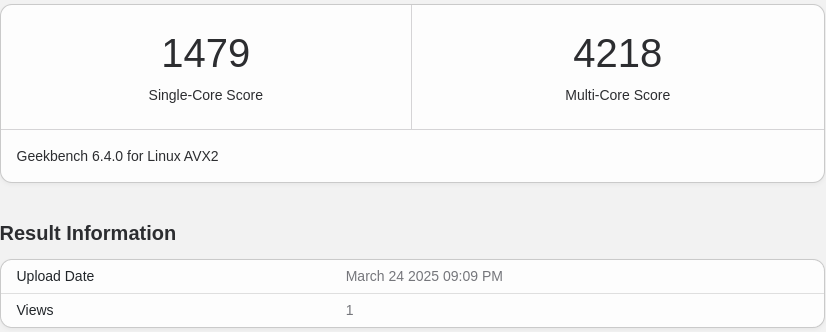
\includegraphics[width=0.6\textwidth]{img/Geekbench.png}
\end{center}



\subsubsection*{x11perf}
Se realizaron varias pruebas con la herramienta \textbf{x11perf}.  
Resultados obtenidos:

\begin{center}
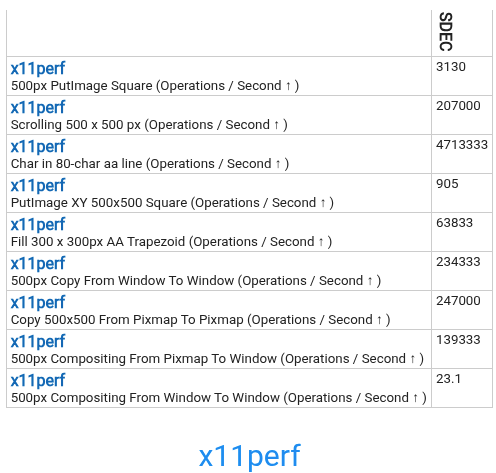
\includegraphics[width=0.6\textwidth]{img/x11perf.png}
\end{center}
La PC muestra un buen rendimiento en operaciones gráficas 2D bajo X11, especialmente en tareas como desplazamiento y renderizado de texto. Con un puntaje alto en pruebas de desplazamiento y dibujo, es adecuada para tareas generales como navegación y edición de texto. Sin embargo, para aplicaciones gráficas más intensivas, el rendimiento podría no ser tan alto como el de sistemas más modernos. En resumen, es suficiente para actividades cotidianas, pero podría quedarse corta en tareas gráficas más exigentes.
\subsubsection*{GLmark2}
Se realizaron varias pruebas con la herramienta \textbf{GLmark2}.  
Resultados obtenidos:

\begin{itemize}
    \item \textbf{GTX 1070}: 6459
\end{itemize}

Resultados de placas mas modernas:

\begin{center}
    \begin{itemize}
        \item \textbf{AMD Radeon RX 6900 XT}: 21869
        \item \textbf{RX6950 XT}: 19262
        \item \textbf{RTX 3060 Ti}: 8436
    \end{itemize}    
\end{center}

Al compararla con las tarjetas gráficas más modernas, la \textbf{GTX 1070} se queda atrás frente a la gama media actual. Esto hace que, para juegos con altos requisitos gráficos, ya esté comenzando a quedar desactualizada.


\subsubsection*{Benchmark de disco con \textbf{fio}}
Se realizó un test de escritura secuencial con la herramienta fio en un disco \textbf{NVMe WD Black}.  
Resultados obtenidos:
\begin{itemize}
    \item \textbf{IOPS}: 274,456
    \item \textbf{Ancho de banda (BW)}: 1069 MiB/s (aproximadamente 1121 MB/s)
    \item \textbf{Latencia promedio de escritura}: 3.44 \textmu s
    \item \textbf{Latencia máxima de escritura}: 111 \textmu s
\end{itemize}

Este rendimiento muestra que el \textbf{NVMe WD Black} ofrece una velocidad de escritura secuencial muy alta, con baja latencia, lo que lo convierte en una excelente opción para tareas que requieren un alto rendimiento en discos.

\subsubsection*{3. Reflexión final}

A pesar de que la PC cumple con las necesidades básicas y las tareas universitarias, como el desarrollo de software, la simulación de sistemas y la ejecución de máquinas virtuales, presenta algunas limitaciones cuando se enfrenta a actividades que requieren un mayor rendimiento, como juegos exigentes y ciertas simulaciones con alto uso de GPU o CPU.

El \textbf{Intel Core i7-7700K}, aunque sigue siendo un procesador decente para tareas generales, ha quedado obsoleto en comparación con los chips más modernos, como el \textbf{AMD Ryzen 5 7600} o el \textbf{Intel Core i3-10100} en cuanto a rendimiento multi-core. Esto se refleja en los benchmarks de Geekbench, donde el rendimiento multi-core del i7 7700K es superado ampliamente por los modelos más nuevos.

Por otro lado, la \textbf{GTX 1070}, a pesar de ser una tarjeta gráfica de gama alta en su momento, ya se muestra limitada para juegos de alto rendimiento gráfico, con resultados que no se comparan con las tarjetas más recientes, como la \textbf{RTX 3060 Ti} o la \textbf{AMD RX 6900 XT}. Esto sugiere que, para juegos exigentes, la tarjeta gráfica está comenzando a quedar desactualizada.

Sin embargo, en cuanto a tareas relacionadas con el \textbf{desarrollo de software} y la \textbf{simulación}, la PC sigue siendo perfectamente funcional. El \textbf{NVMe WD Black} demuestra un rendimiento excelente en cuanto a velocidad de lectura y escritura secuencial, lo que resulta en una experiencia fluida en tareas de compilación y manejo de grandes volúmenes de datos. Además, la memoria RAM y el rendimiento de la CPU son adecuados para proyectos universitarios y uso cotidiano.

En conclusión, la PC cumple perfectamente con las necesidades para actividades académicas y de desarrollo básico, pero presenta limitaciones cuando se requieren altos niveles de rendimiento gráfico o de procesamiento paralelo. Para tareas más exigentes, sería recomendable considerar una actualización de la \textbf{tarjeta gráfica} y la \textbf{CPU}, aunque para actividades más simples y universitarias, la máquina sigue siendo una herramienta eficiente.


\newpage

\subsection{Resultados PC Genaro}
\subsubsection*{1. Uso cotidiano de la PC}
La PC se utiliza principalmente para desarrollo de software y ejecución de simulaciones. Los programas y entornos utilizados incluyen:
\begin{itemize}
    \item \textbf{Desarrollo de software:} Visual Studio Code, PyCharm, Eclipse.
    \item \textbf{Simulaciones:} MATLAB, Simulink, ANSYS.
    \item \textbf{Otros:} Navegación web con múltiples pestañas, edición de documentos en LaTeX.
\end{itemize}

\subsubsection*{2. Tareas y benchmarks representativos}

A continuación se presenta una tabla con algunas tareas frecuentes relacionadas con simulaciones y desarrollo de código, junto con el benchmark que mejor representa cada una.

\begin{center}
\begin{tabular}{|p{7cm}|p{7cm}|}
\hline
\textbf{Tarea} & \textbf{Benchmark representativo} \\
\hline
Compilar proyectos grandes en C/C++ & Geekbench o Cinebench (CPU multi-core) \\
\hline
Ejecución de simulaciones en MATLAB/Simulink & SPEC CPU2017 \\
\hline
Desarrollo de software en entornos pesados (e.g., PyCharm, Eclipse) & PassMark CPU \\
\hline
Análisis de datos y cálculos intensivos en Python & Geekbench (CPU single-core) \\
\hline
\end{tabular}
\end{center}

\subsubsection*{3. Reflexión final}
En términos generales, la PC cumple con los requerimientos diarios para el desarrollo de software y la ejecución de simulaciones. Sin embargo, se ha identificado que el rendimiento de la CPU puede convertirse en un cuello de botella durante la ejecución de simulaciones complejas y la compilación de proyectos grandes. 

Existe interés en evaluar y mejorar el rendimiento en estas tareas específicas, por lo que se considerará realizar actualizaciones de hardware, como la incorporación de un procesador más potente o la ampliación de la memoria RAM, para optimizar el rendimiento.


\section{Conclusiones}
Conclusiones del trabajo realizado.

\end{document}
